
\parindent 0in
\parskip 0.1in

{\bf Title:  Reduced Order Modeling of heat and fluid flow: Multi-scale modeling of advanced reactors to enable faster deployment }

{\bf Technical work scope identification: M\&S 1 }

{\bf PI:}
Paul Fischer \\
Department of Computer Science \\
Department of Mechanical Science \& Engineering \\
University of Illinois, Urbana-Champaign \\

{\bf co-PIs:}
Elia Merzari, Pennsylvania State University, \\
Dillon Shaver, Argonne National Laboratory \\

\section{Project Summary}

% \begin{itemize}
% \item
% A summary of the proposed project, including a description of the project and a
% {\em clear explanation of its importance and relevance to the objectives in Part I
% Section A.}
% \item
% Major deliverables and outcomes the R\&D will produce.
% \item
% Timeframe of execution: October 1, 2023--September 30, 2026
% \end{itemize}

We seek \textbf{to develop novel multi-scale algorithmic approaches for the
simulation of heat and fluid flow in advanced reactors}. The methods, which
leverage recent advances in hardware and reduced order modeling approaches,
will enable fast-running simulations of vastly accelerated speed, while
maintaining accuracy comparable to high-fidelity methods such Large Eddy
Simulation and Direct Numerical Simulation. These methods will allow to perform
parameter sweeps to assess uncertainty and develop closures. They will also
enable, for the first time to perform high fidelity simulation of transients.

Several  advanced reactors concepts are currently being pursued in the United
States, with dozens of companies proposing unique designs. Crucial for their
deployment is the analysis of  reactor transients (e.g., a protected loss of
flow): an essential part of the evaluation of thermal margins and the overall
safety case.  In most cases, licensing will be pursued with established
methods, based on lumped parameter system codes (e.g., SAM \cite{hu2021}).
However, these codes require adequate closures, that are typically obtained
empirically and require extensive validation. Furthermore, the methods are
characterized by high level of uncertainty when dealing with complex
three-dimensional turbulent flow, especially in the presence of large
enclosures, mixed convection and thermal stratification. High-fidelity
simulation on the other hand remains prohibitively expensive, especially for
large parameter sweeps or for the simulation of nuclear transients, and data
remains sparse.

Moreover, as the advanced reactor industry matures and moves past demonstration
projects, economics will become a larger and larger driver. This will very
likely push vendors to seek to maximize the economic potential (e.g., higher
power output, higher temperature for process heat, reduced capital cost),
especially as new materials and fuels are introduced. These goals will benefit
from radically improved methods to assess thermal margins that push toward high
fidelity. \textbf{This proposal seeks to develop radically novel algorithmic
approaches to the simulation of advanced reactors, with an unprecedented level
of fidelity, enabling transformative design approaches and improved economics.}
In particular we aim to:
\begin{enumerate}
%
   \item \textit{Enable the simulation of large parameter sweeps using reduced
   order models developed over a subset of the parameter space.} This approach
   will allow to assess uncertainty of system-level approaches and to develop
   closures.
%
   \item \textit{Enable the simulation of accelerate simulation of transients }
   This approach will allow to assess lower resolution approaches in conjunction
   with experimental data for the simulation of transient.
\end{enumerate}
As a demonstration application we choose the simulation of Sodium Fast Reactor
fuel assemblies under steady-state and transient conditions. \textit{ We
emphasize that the methods developed will apply to a broad range of advanced
reactor applications.} An overview of the project is provided in Figure~\ref{f:01}.

\begin{figure}[h!]
    \centering
    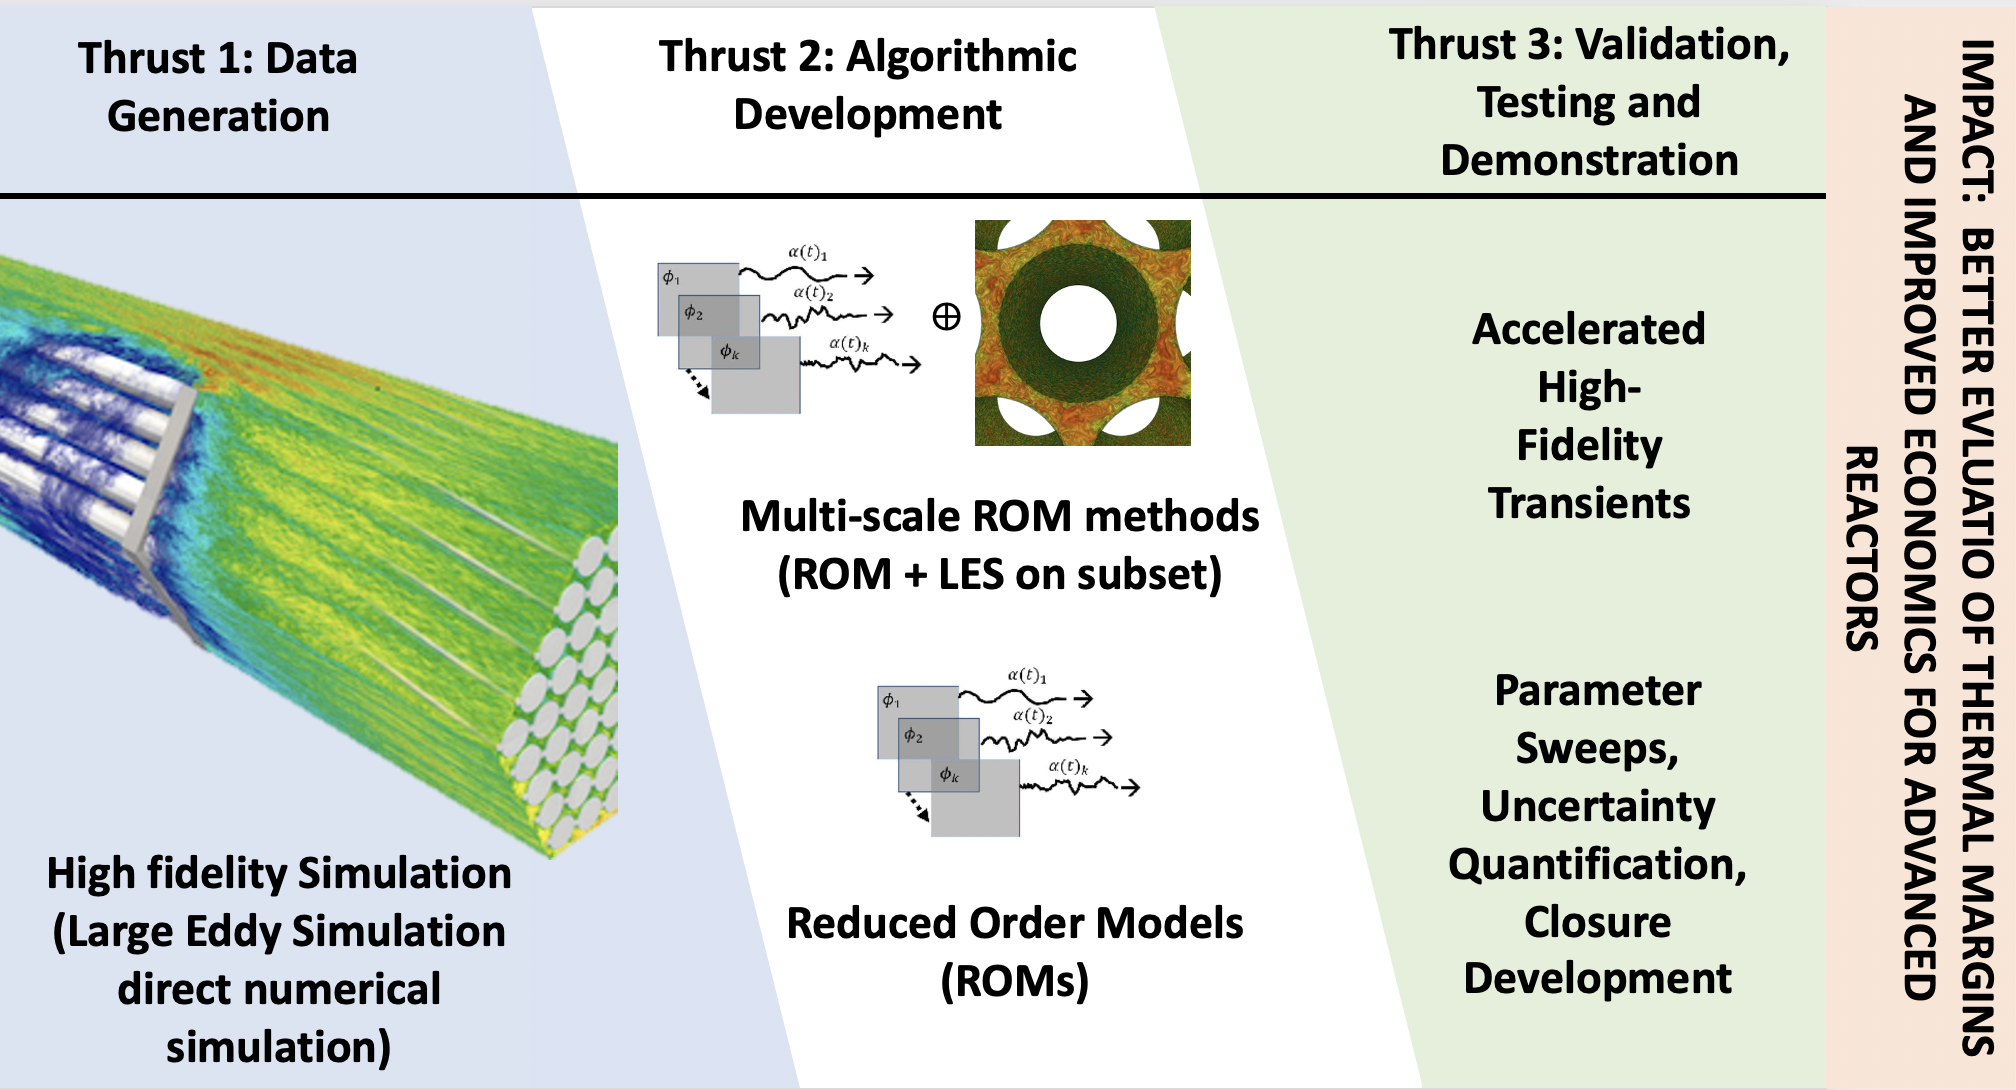
\includegraphics[width = 0.85\textwidth]{figs/fig1.PNG}
    \caption{Overview of Project with three thrusts: Data generation, algorithmic development and validation/demonstration.}
    \label{f:01}
\end{figure}


\section{Project Motivation and Technical Objectives}

We propose to leverage current hardware, software, and algorithmic developments
to radically enhance thermal-hydraulic analysis capabilities.  The work will
entail combining advanced simulations on DOE's exascale computing platforms
with modern data analysis methods that effectively compress these
first-principle data to efficient exploratory tools based on reduced-order
models (ROMs) and machine learning (ML).

Recent breakthroughs in computational hardware and software have the potential
to significantly improve predictive capabilities for reactor thermal hydraulics
(TH).  The Department of Energy is in the process of standing up three exascale
computing platforms: Frontier at ORNL, El Capitan at LLNL, and Aurora at ANL.
We have recently demonstrated that it is possible to simulate a single flow
through time for the thermal-hydraulics of a full pebble-bed reactor core
(352,000 pebbles) in just six hours of wall-clock time on the {\em
pre}-exascale machine, Summit, at ORNL \cite{sc22}.   This is an impressive
acheivement as it involves a quarter-trillion degrees-of-freedom, executing a
0.3 seconds per step.  This problem is relatively small by exascale standards,
so it will be possible to explore multiple configurations in this space within
a single annual allocation, which will make it possible to consider parameter
exploration that is critical for analysis and design.

PICTURE OF PEBBLE BED HERE

CITE OTHER PAPERS BY ELIA \& team

Mention NRC CRAB

Pointwise exploration of parameter spaces, however, is not as efficient as being
able to leverage expensive exascale simulations (known as {\em full-order
models}) to generate inexpensive surrogates to explore a broader parametric
space at low cost.    These surrogates can be generated through {\em reduced-order
models} (ROMs) using some type of Galerkin projection or in combination with
machine learning (ML).   In either case, the idea is to leverage high-fidelity
data generated on pre-exascale or exascale platforms to allow reactor designers
to rapidly explore thermal-hydraulics responses over a significant parametric
space.

The software development to bring this vision to fruition is well underway.
On the exascale side, Nek5000/RS is capable of strong-scaling to tens-of-thousands
of GPUs with only 2--3M points per GPU, so that it can effectively leverage
the high processor counts of DOE's leadership computers.  Currently, Nek5000/RS
sustains $\approx 1$ TFLOPS ($10^{12}$ floating point operations per second)
{\em per GPU} on Summit and Crusher, two of DOE's pre-exascale platforms.
The overall performance is 3$\times$ that observed for the IBM BG/Q, Mira,
where Nek5000 has scaled to over a million MPI ranks.   Reactor simulation
milestones on Mira and Summit include (FIG FIG FIG, cite cite cite).

On the modeling side...  cite: \\
.Elia ROMs \\
.recent papers supported under NEUP. \\
.other authors

In addition to ROMs, there has been significant progress in applying
ML to fluid simulation problems, including: \\
Vinuesa, others, ...


Elia: WHAT PROBLEM(s) SHOULD WE LOOK AT ?

Paul: How will we use ML

Paul: How will we push ROM/pMOR ?









New things:

ROM / pMOR

compressed I/O

















\section{Introduction}

SN-1: THERMAL HYDRAULICS AND HEAT TRANSFER (FEDERAL POC – JENNA PAYNE) \\
(ELIGIBLE TO LEAD: UNIVERSITIES ONLY) \\
(UP TO 3 YEARS AND \$500,000) \\

Maintaining fundamental skills and knowledge in key nuclear engineering topics
is important to maintain and establish research excellence and expertise.
Sub-topic areas are intentionally broad to allow for flexibility in response. A
response should address innovative research in the identified area and could
include any aspect (experiments, modeling, etc.) that is necessary to
accomplish the proposed scope.
\\

{\bf Pre-Applications due 10/11/22:}
R\&D/NSUF Pre-Applications (Mandatory except for IRPs) Due Date: October 11, 2022 at 7:00 p.m. ET


Pre-Applications must include a list of publications
that resulted from previous NSUF supported projects.


\section{Pre-Application}


{\bf D. CONTENT AND FORM OF ALL PRE-APPLICATIONS (Mandatory except for IRPs)}

Pre-Applications are a mandatory requirement for R\&D and NSUF Access Only
Projects (in Appendices A and C of this CINR FOA) for U.S. University-,
National Laboratory-, or Industry- led projects. Pre-Applications must be
submitted by the date and time specified in Part IV, Section G.2 of this CINR
FOA.  The PI and named collaborators identified in the Pre-Application may not
be changed in the Full Application without adequate justification and consent
of the Contracting Officer.  The following information shall be provided for
all Pre-Applications:

{\bf D.1 Pre-Application Narrative} (5 pages)

Applicant shall provide a narrative that addresses the specific information below:

• Title of project.

• Technical work scope identification (e.g., NM-1). The PI is responsible for
selecting the appropriate work scope, and this may not be changed between the
Pre-Application and Full Application.

• Name of PI(s) and associated organization(s).

• A summary of the proposed project, including a description of the project and
a clear explanation of its importance and relevance to the objectives in Part I
Section A.

• Major deliverables and outcomes the R\&D will produce.

• Estimated cost of project (not including value of any NSUF access).

• Timeframe for execution of proposed project (specify the time period for R\&D,
one-, two-, or three-year period or up to seven years for NSUF).

• Specific facilities and equipment access requirements (for the NSUF access portion only).

• A clear and concise summary of the readiness of the project for NSUF access
(as described in Part I, Section B.3.1 of this CINR FOA).

• Proprietary data, such as chemical composition or physical properties of a
material, that the applicant wishes to protect during the irradiation or PIE
phase of the project. This may negatively impact the selection of the project.
Pages outside the specified page limits and font size, including references,
will be redacted and unavailable for evaluators to review.

o 5-page limit, 11-point font.  Name File: 2023 Pre-Application Narrative
“Insert ID \#”

{\bf D.2 Benefit of Collaboration} (4 pages)

Applicant shall provide a narrative that includes an explanation of the
contribution that will be made by the collaborating organizations and/or
facilities to be utilized. It may contain brief biographies of staff and
descriptions of the facilities wherein the research will be conducted. Please
indicate within this section whether the application has benefit or influence
on other ongoing or proposed NE R\&D projects (e.g., modeling and simulation in
one application and effect validation in a separate application).

This document is required unless the application only has a single principal
investigator.

Pages outside the specified page limits and font size, including references,
will be redacted and unavailable for evaluators to review.

o 4-page limit, 11-point font.

Name File: 2023 RPA Benefit of Collaboration “Insert ID \#”

{\bf D.3 Publications} (Past NEUP/NEET/NSUF Publications)

Applications must include a list of publications that resulted from previous NE
(NEUP, NEET, NSUF) funded projects. A reference to the project that supported
each publication should be included. If the PI has not led an NE (NEUP, NEET,
NSUF) project, this document is not required.

o No page limit.

Name File: 2023 RPA NE Supported Publications “Insert ID \#”

{\bf D.4 Principal Investigator Vitae} (LEAD PI ONLY, 2 pages)

The lead PI shall provide a brief curriculum vitae (CV) that lists the
following:

• Contact information.

• Education and Training: provide institution, major/area, degree, and year for
undergraduate, graduate, and postdoctoral training.

Fiscal Year 2023 Consolidated Innovative Nuclear Research PART IV

• Research and Professional Experience: beginning with the current position
list, in chronological order (newest to oldest), professional/academic
positions with a brief description.

• Publications: Provide a list of up to 10 publications most closely related to
the proposed project. For each publication, identify the names of all authors
(in the same sequence in which they appear in the publication), the article
title, book or journal title, volume number, page numbers, year of publication,
and website address if available electronically.

• Patents, copyrights, and software systems developed may be provided in
addition to or substituted for publications.

• Synergistic Activities: List no more than five professional and scholarly
activities related to the effort proposed.

Pages outside the specified page limits and font size, including references,
will be redacted and unavailable for evaluators to review.

o 2-page limit, 11-point font.

Name File: 2023 RPA “Last Name of Individual” “Insert ID \#”

{\bf D.5 Collaborators}

A collaborator is an individual who makes a defined, material contribution that
is critical to the success of the project and/or contributing to joint
publications. Any individual appearing in the project summary, technical
narrative, benefit of collaboration, coordination and management plan, or
budget documents should be listed as a collaborator directly on the application
form. The applicant must have the full consent of all collaborators prior to
submitting an application. Any individuals that do not meet these criteria
should not be listed as collaborators on the application.


{\bf D.6 Agreement Requirements}

Institutions will be expected to follow Quality Assurance (QA) principles and
requirements in conducting R\&D activities. If the application is successful,
the integrity of R\&D products and their usability by NE is predicated on
meeting QA requirements, as they apply to a specific scope of work and
associated deliverables. Further, each institution serving as a team member to
the proposed project shall be identified in the Pre-Application with its
commitment made to collaborate in the CINR FOA process.

If applicable, access to NSUF capabilities will require agreement and final
signature to the User Agreement (copy provided in Part IX, Appendix E of this
CINR FOA). The terms and conditions of the User Agreement are non-negotiable,
and failure to accept the terms and conditions of the User Agreement will
terminate processing and review of NSUF applications. To ensure compliance
throughout the application review process, applicants must state, during the
NSUF Access Only and Full Application submission processes, that the User
Agreement has been read, understood, and the terms and conditions are accepted.
Further, submission of a NSUF supported Pre-Application and a Full Application
indicates the applicant will comply and agree to the terms and conditions of
the User Agreement. Upon award of an Page 25 of 107

Fiscal Year 2023 Consolidated Innovative Nuclear Research PART IV NSUF
supported project, the User Agreement must be signed before activities will
begin on the project. Failure to sign the non-negotiable User Agreement within
30 days of receipt of the User Agreement may result in cancellation of an
awarded project.
